\documentclass[legalpaper,11pt]{article}

%\pagestyle{empty}


%%%%%%%%%%%%%%%%%%%%%%%%%%%%%%% Paquetes %%%%%%%%%%%%%%%%%%%%%%%%%%%%%%%%%%%

\usepackage[ansinew]{inputenc}
\usepackage[spanish]{babel}
\usepackage[mathcal]{euscript}
\usepackage{amsmath,amsfonts,amssymb,theorem,latexsym,mathrsfs, %hyperref,
            epsfig, multicol,anysize,graphicx,enumitem,mdwlist}
\usepackage{graphicx}  
\usepackage{ragged2e}  
\usepackage{float}        


%%%%%%%%%%%%%%%%%%%%%%%%%%%%%%%%%%%%%%%%%%%%%%%%%%%%%%%%%%%%%%%%%%%%%%%%%%%%


%%%%%%%%%%%%%%%%%%%%%%%%%%%%%%% M�rgenes %%%%%%%%%%%%%%%%%%%%%%%%%%%%%%%%%%%

\marginsize{1cm}{1cm}{0.2cm}{1cm}

%\marginsize{izquierdo}{derecho}{arriba}{abajo}

%%%%%%%%%%%%%%%%%%%%%%%%%%%%%%%%%%%%%%%%%%%%%%%%%%%%%%%%%%%%%%%%%%%%%%%%%%%%


%%%%%%%%%%%%%%%%%%%%%%%%%%%%% Definiciones %%%%%%%%%%%%%%%%%%%%%%%%%%%%%%%%%

\def\r{\mathbb{R}}
\def\n{\mathbb{N}}
\def\q{\mathbb{Q}}
\def\c{\mathbb{C}}
\def\z{\mathbb{Z}}

\def\sen{\mathop{\mbox{\normalfont sen}}\nolimits}
\def\intt{\mathop{\mbox{\normalfont int}}\nolimits}
\def\diag{\mathop{\mbox{\normalfont diag}}\nolimits}
\def\arcsen{\mathop{\mbox{\normalfont arcsen}}\nolimits}
\def\ln{\mathop{\mbox{\normalfont ln}}\nolimits}
\def\tr{\mathop{\mbox{\normalfont tr}}\nolimits}

%%%%%%%%%%%%%%%%%%%%%%%%%%%%%%%%%%%%%%%%%%%%%%%%%%%%%%%%%%%%%%%%%%%%%%%%%%%%

\begin{document}

%%%%%%%%%%%%%%%%%%%%%%%%%%%% Encabezado %%%%%%%%%%%%%%%%%%%%%%%%%%%%%%%%%%%%

\begin{minipage}{0.11\linewidth}

\includegraphics[width=20mm]{escudo.jpg}
\end{minipage}
\begin{minipage}{0.78\linewidth}
\centerline{UNIVERSIDAD DE ANTIOQUIA}
\centerline{Facultad de Ciencias Exactas y Naturales}
\centerline{Instituto de Matem�ticas}
\centerline{Final - Series de Tiempo I}
%\centerline{Taller $\#$ 1}
\end{minipage}

\vspace{3mm}

\leftline{Profesor: Duv�n Cata�o}


\vspace{5mm}


\begin{enumerate}

\item Suppose we would like to predict a single stationary series $x_t$ with zero mean and autocorrelation function $\gamma(h)$ at some time in the future, say, $t + l,$ for $l > 0.$
\begin{enumerate}
\item If we predict using only $x_t$ and some scale multiplier $A$, show that the mean-square prediction error 

$$MSE(A) = \mathbb{E}[(x_{t+l}-Ax_t)^2]$$

is minimized by the value
$$ A = \rho(l).$$

\item Show that the minimum mean-square prediction error is 
$$MSE(A) = \gamma(0)[1 - \rho^2(l)].$$

\item Show that if $x_{t+l} =Ax_t,$ then $\rho(l)=1$ if $A>0$, and $\rho(l)=-1$ if $A<0.$
\end{enumerate}

\newpage

\item Una serie de 400 observaciones present{\'o} los siguientes resultados:

\begin{table}[htdp]
\begin{center}\begin{tabular}{c|ccccccc}
$h$ & 1 & 2 & 3 & 4 & 5 & 6 & 7   \\
\hline
$\phi_{hh}$ & 0.8 & -0.5 & 0.07 & -0,02 & -0,01 & 0.05 & 0.04 
\end{tabular} 
\end{center}
\label{defaulttable}
\end{table} 

con $\bar{x}_t=8$ y $\mu_0=9.$

\begin{enumerate}
\item Explique por qu\'e podemos ajustar a la serie un modelo AR$(2).$
\item Obtenga las estimativas $\hat{\phi_1}$ y $\hat{\phi_2}$ del modelo AR$(2)$ utilizando las ecuaciones de Yule-Walker.
\item Verifique que el modelo ajustado satisface las condiciones de estacionaridad.
\item Usando $\hat{\phi_1}$ y $\hat{\phi_2}$ como verdaderos, describa el comportamiento general de la ACF de ese proceso. 
%\item Obtenga los pron\'osticos para los pr\'oximos 4 periodos.
\end{enumerate}

\newpage

\item Suponga que el modelo $(1-B^4)x_t=a_t+a_{t-1}-0,5a_{t-4},$ donde $\sigma_a^2=2,25$, fue ajustado a las observaciones de una serie de datos trimestrales con una muestra de $T=100.$\\
Suponga que las observaciones y residuos de los \'ultimos cuatro trimestres son dadas por:

\begin{table}[htdp]
\begin{center}\begin{tabular}{c|cccc}
Trimestre & I & II & III & IV   \\
\hline
$x_t$ & 124 & 121 & 129 & 139 \\
\hline
$a_t$ & 2 & -1 & 1 & 3 \\

\end{tabular} 
\end{center}
\label{defaulttable}
\end{table} 

\begin{enumerate}
\item Encuentre las predicciones $x_{100}(l)$, para $l=1,2,3,4.$ 
\item Construya los intervalos de predicci\'on con $\alpha=0,05.$
\end{enumerate}

\newpage

\item Suponga que el modelo ajustado para $x_t$ ha sido 
$$x_t-x_{t-1}=(1-0,5B)b_t,$$
pero los residuos $b_t$ no son aleatorios. Si el modelo posteriormente identificado para $b_t$ fue un ARIMA$(0,1,1),$ con $\theta=-0,8$, ?`cu\'al es el modelo que debemos considerar para $x_t$?


\end{enumerate}

\end{document}


% \begin{figure}[H]
%  \centering
%  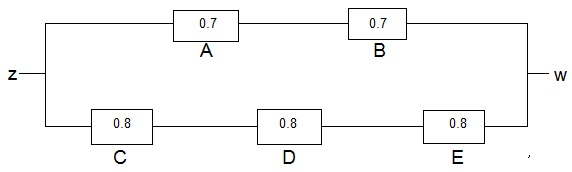
\includegraphics[width=.50\textwidth]{tab3}
% \end{figure}